% ****** Start of file aipsamp.tex ******
%
%   This file is part of the AIP files in the AIP distribution for REVTeX 4.
%   Version 4.1 of REVTeX, October 2009
%
%   Copyright (c) 2009 American Institute of Physics.
%
%   See the AIP README file for restrictions and more information.
%
% TeX'ing this file requires that you have AMS-LaTeX 2.0 installed
% as well as the rest of the prerequisites for REVTeX 4.1
% 
% It also requires running BibTeX. The commands are as follows:
%
%  1)  latex  aipsamp
%  2)  bibtex aipsamp
%  3)  latex  aipsamp
%  4)  latex  aipsamp
%
% Use this file as a source of example code for your aip document.
% Use the file aiptemplate.tex as a template for your document.
\documentclass[%
 aip,
% jmp,
% bmf,
% sd,
% rsi,
 amsmath,amssymb,
%preprint,%
 reprint,
%author-year,%
%author-numerical,%
% Conference Proceedings
]{revtex4-1}
\usepackage[normalem]{ulem}
\usepackage{graphicx}% Include figure files
\usepackage{dcolumn}% Align table columns on decimal point
\usepackage{bm}% bold math
%\usepackage[mathlines]{lineno}% Enable numbering of text and display math
%\linenumbers\relax % Commence numbering lines

\usepackage[utf8]{inputenc}
\usepackage[T1]{fontenc}
\usepackage{mathptmx}
\usepackage{etoolbox}

  %-----ADDED LATER---
\usepackage{mathtools,amssymb}
\usepackage[abs]{overpic}
\usepackage{xcolor,varwidth}
\usepackage{tikz}
\newcommand*\circled[1]{\tikz[baseline=(char.base)]{
		\node[shape=circle,draw,inner sep=1pt] (char) {#1};}}
\usepackage{setspace} 
%%%%Author definitions
%\def\tsc#1{\csdef{#1}{\textsc{\lowercase{#1}}\xspace}}
%\tsc{WGM}
%\tsc{QE}
%\tsc{EP}
%\tsc{PMS}
%\tsc{BEC}
%\tsc{DE}
%%%%
\usepackage{lineno}

%% Apr 2021: AIP requests that the corresponding 
%% email to be moved after the affiliations
\makeatletter
\def\@email#1#2{%
 \endgroup
 \patchcmd{\titleblock@produce}
  {\frontmatter@RRAPformat}
  {\frontmatter@RRAPformat{\produce@RRAP{*#1\href{mailto:#2}{#2}}}\frontmatter@RRAPformat}
  {}{}
  
}%
\makeatother
\begin{document}

\preprint{AIP/123-QED}

\title[]{Flexible structures enhance fluid mixing in a channel flow}
\author{Gaurav Singh*}
% \altaffiliation[Also at]{Advanced Technology and Development Centre}%Lines break automatically or can be forced with \\
 \affiliation{Advanced Technology and Development Centre, Indian Institute of Technology Kharagpur, West Bengal, India -721302}
  \email{thegauravonline@gmail.com}
  
\author{Arahata Senapati}%
\affiliation{Advanced Technology and Development Centre, Indian Institute of Technology Kharagpur, West Bengal, India -721302}

\author{Abhishek Sharma}
\affiliation{Department of Chemical Engineering, Indian Institute of Technology Kharagpur, West Bengal, India -721302}
\author{Arnab Atta}
\affiliation{%
	Department of Chemical Engineering, Indian Institute of Technology Kharagpur, West Bengal, India -721302}
	\author{Rajaram Lakkaraju}
	% \homepage{http://www.Second.institution.edu/~Charlie.Author.}
	\affiliation{Turbulent Interfaces And Dispersion (TRIAD) Group, Department of Mechanical Engineering, Indian Institute of Technology Kharagpur, West Bengal, India -721302 }
%	  \email{rajaram.lv@gmail.com}

\date{\today}% It is always \today, today,
             %  but any date may be explicitly specified

\begin{abstract}
 Early fluid mixing in channel flows without incurring much drop in the pressure head is desired in industrial applications. In this work, we show the enhanced mixing performance in a channel flow by using wall-mounted flexible plates as obstacles. Using fluid-structure-scalar interaction simulations, we investigate the oscillations of the flexible plates under the flow, which serve as vortex generator and help increase the mixing. The channel flow consists of a scalar field with two distinct concentrations, which are initially separated across the channel and inter-mix over the time due to several scales of vortical structures. We have used the `Mixing Index' and mechanical `Head Loss' metrics along the channel length to assess the mixing quality when plates with different flexibility (characterized by the Cauchy number, $Ca$) are used. We have also investigated the effect of pulsatile fluid inlet (quantified by the Strouhal number, $St_f$) on mixing. To investigate the efficacy of our setup based on the equivalent mixing and head loss in an empty channel case (with no obstacles) and deduced a comprehensive criteria called `co-efficient of performance'. On aggregating all our cases on this scale, we conclude that the case with $Ca=0.06$ with $St_f=32$ offers the best mixing performance downstream in the channel when estimated against the head loss as the cost. A major conclusive takeaway from this work is that the plates with increased flexibility result in better mixing outcomes, and using a pulsatile inlet can marginally enhance this performance in certain instances. 
\end{abstract}

\maketitle

\setstretch{1.6}
\section{Inroduction}
\label{sec:headings}
Fluid mixing plays a crucial role as a pretreatment process in various industrial applications, including fuel emulsification in the petrochemical sector, the blending of raw materials in the food industry, and the mixing of different chemical components in chemical engineering domains \citep{Peterwitz2021,Wang2021, Nunez-Flores2020, Yeh2015}. To enhance the mixing of fluids in a channel flow, a commonly employed strategy involves modifying the structural and dimensional aspects of the mixing channels. For instance, \cite{Kim2011} introduced ribbed configurations of varying dimensions into micromixers, resulting in a significant 32.2\% reduction in the mixing path. \cite{Yang2015} developed a channel design inspired by the three-dimensional Tesla design, demonstrating a robust mixing index of $0.97$ (where $0$ meant no-mixing and $1$ meant perfect-mixing case) within a Reynolds number range of $0.1$ to $100$. Additional studies, such as those by \cite{Chen2016}, illustrated that topological alterations in serpentine mixer channels could induce chaotic convective motions and molecular diffusion, consequently enhancing mixing outcomes. \cite{Lobasov2018} provided valuable insights into the relationship between channel geometry and the critical Reynolds number that dictates the transition from stable symmetric to asymmetric flow regimes, with the latter resulting in significant improvements in mixing efficiency.

Apart from modifications in channel design, the incorporation of vortex generators within mixing channels has emerged as a key approach to enhancing the mixing process \citep{Ali2015,Khatavkar2007,Dadvand2019,Ali2016,Hsiao2014,Hosseini2021,Van_Loon2007,Eizadi2022}. A fundamental method within this approach involves the placement of shaped obstructions that act as catalysts for Kármán vortex streets and flow agitation, thereby facilitating enhanced mixing \citep{Abdelhamid2021,Yadav2021,Jing2022,Yu2017}. However, in the case of such vortex generators, the vortex mainly concentrates in the small wake zone behind the obstacle, resulting in weak mixing near the channel wall, especially when the channel dimension greatly exceeds the obstacle size \citep{Wang2020}. A promising solution to this limitation is to employ flexible structures as vortex generators \citep{Chen2020,Park2019,Saleh2019,Zhao2020,Pfister2020}. When fluid flows over flexible structures, it induces hydrodynamic and structural instabilities that manifest as various flow scales, self-induced structural oscillations, and acoustic noise \citep{Balachandar1999, Zhang2000, Mahadevan2004, Vandenberghe2004, Shelley2011}. These instabilities arise when there is an imbalance between destabilizing hydrodynamic forces and stabilizing elastic restoring forces \citep{Taneda1968, Zhang2000, Watanabe2002, Eloy2008, ZhuPeskin2002, Alben2008}. Typically, such instabilities lead to flow agitation in a channel, which is highly advantageous in applications like micro-total analysis \citep{Manz2002} and other applications such as heat exchangers or chemical reactors where enhanced mixing is crucial. In addition to these strategies, leveraging inertial effects in fluid mixing within a channel is also a popular method \citep{Carlo2009,Carlo2007} such as utilizing unsteady time-periodic flow methods or pulsatile flows \citep{Cai2017}, to take advantage of time-varying pressure, velocity, shear stresses. These strategies have also been applied for enhanced separation and mixing \citep{Ward2015}, microdroplet pinch-off and control \citep{Zhu2017, SENAPATI2019}, efficient on-chip process automation, and clog mitigation \citep{Mehendale2018}.

Drawing inspiration from previous research on microchannel flow \cite{Khatvakar2007, LambertRangel2010, Gleeson2005, Pathak2012, Kim2010, Stone2001, Stone2004}, our study involves two-dimensional numerical simulations to investigate the flow past two flexible plates, each occupying nearly half of the channel height and mounted on the opposite channel walls (as shown in Figure \ref{fig:schematic}). Our investigation focuses on an approach to inertial micromixing that capitalizes on the flow-induced bending and oscillations of the flexible plates to enhance mixing. We also examine the impact of wall-mounted plates on fluid mixing in a channel under both steady inlet conditions and pulsatile flow inlets at various periodicities. The objective is to determine whether flexible wall-mounted plates outperform rigid ones in the Reynolds number regime of $\mathcal{O}(100)$. This study aims to assess optimal fluid mixing and the associated head loss in the channel to identify the optimal configuration that offers the best mixing performance.

\begin{figure}
	\begin{center}
		\begin{minipage}[c]{1\linewidth}	
			\begin{overpic}[width=1\linewidth]{Figures/Schematic-02.png}
				\put(80,97){{\parbox{1\linewidth}{$\phi = 1$}}}	
				\put(80,82){{\parbox{1\linewidth}{$\phi = 0$}}}	
				\put(-56,-4){{\parbox{1\linewidth}{$Re/Re_s$}}}	
				\put(-108,36){{\parbox{1\linewidth}{\rotatebox{90}{$y/h$}}}}	
			\end{overpic}
		\end{minipage}
	\end{center}
	\caption{Schematic of the flow past wall-mounted flexible plates. Flow enters from the inlet (left), passes through the gap between the two oppositely mounted plates, and leaves the channel from the outlet (right). The channel is pre-filled with a scalar concentration field $\phi$, which is distinctly separated as $\phi=1$ on top and $\phi=0$ in the bottom half of the channel as an initial condition. The inlet flow is considered as pulsatile, and the flow oscillation is shown in the bottom panel. Also, a zoom-in of the typical mesh grid used in the simulation is shown.}
	\label{fig:schematic}
\end{figure}


\section{Mathematical formulation and computational setup}\label{sec:maths}
A schematic of our model as a two-dimensional channel geometry of height $h$ and length $14h$ is shown in Fig. \ref{fig:schematic}. Two flexible plates, each of length $l $$\approx$$ 0.5h$ (0.425h), are fixed on the opposite walls at a distance of $2h$ from the channel inlet. A gap of $0.15h$ is spared between the tip edges of the two plates to prevent frictional effects as suggested in \cite{ Zenit2015} and also to facilitate numerical ease. The chosen geometry is inspired by the works of \cite{ Zenit2014, Zenit2015, Zenit2016}, where flow past one flexible plate mounted on a channel wall is studied. Our model is a symmetric form of the same as it employs two wall-mounted plates. The thickness and width of each plate are $b = 0.05h$ and $w=0.125h$ (into the plane), respectively. A flow enters from the left, interacts with the wall-mounted structures and forms vortices into the downstream, generating intricate flow features. We have carried out the fluid (incompressible and Newtonian) and structure (linear elastic) interaction simulations in this geometry using a partitioned approach, where the fluid and solid solvers are run separately, and their solutions are exchanged. The mathematical framework consists of the Navier-Stokes equations for the fluid and the equations of motion for the solid, which are formulated using the Arbitrary Lagrangian-Eulerian (ALE) framework~\cite{Nguyen2010, Slone2002, CampbellPaterson2011}. 
The governing equations for the mass and momentum conservation for the fluids and the structural deformation are,
\begin{equation*}
	\nabla\cdot\left[(\mathbf{u}_f-\mathbf{u}_m)\right] = 0,
	\end{equation*}\vspace{-1.25cm}
\begin{equation*}
	{\partial\mathbf{u}_f\over\partial t} + \left[(\mathbf{u}_f-\mathbf{u}_m) \cdot\mathbf{\nabla}\right]\mathbf{u}_f = -\nabla p+\frac{1}{Re}\nabla^2\mathbf{u}_f,
\end{equation*}\vspace{-1.25cm}
\begin{equation*}
	\rho_s{\partial^2\mathbf{u}_s\over\partial t^2} = \mathbf{\nabla}\cdot\mathbf{\boldsymbol{\sigma}}_s
\end{equation*}
where $\mathbf{u}_f=(u_x,u_y)$ is the flow velocity, $\mathbf{u}_m$ is the mesh velocity, $p$ is the pressure, $\rho_s$ is the structure density, $\mathbf{u}_s$ is the structural displacement, $t$ is the time and $\sigma_s$ is the Cauchy stress tensor. The operator $\frac{\partial}{\partial t}$ represents the time derivative, and $\nabla\equiv\left(\frac{\partial}{\partial x},\frac{\partial}{\partial y}\right)$ is the spatial gradient, and $\nabla^2$ is the Laplacian operator. $Re$ is the Reynolds number i.e., $Re=Uh/\nu_f$ where $U$ is the mean inlet flow velocity, and $\nu_f$ is the fluid kinematic viscosity. The subscripts $_f$, $_s$, and $_m$ correspond to fluid, solid, and mesh, respectively. As the plates' deform under the fluid load, the strain rate is defined as $\boldsymbol{\varepsilon}_s={1\over2}[(\mathbf{\nabla}\mathbf{u}_s+\mathbf{\nabla}\mathbf{u}_s^T)+(\mathbf{\nabla}\mathbf{u}_s - \mathbf{\nabla}\mathbf{u}_s^T)]$. The stress and the strain tensors are related by $\boldsymbol{\sigma}_s=2\mu_s \boldsymbol{\varepsilon}_s+\lambda( \mathbf{\nabla}\cdot\mathbf{u}_s)\mathcal{I}$, where $\mu_s=\mathcal{E}/[2(1+\kappa)]$ and $\lambda=\kappa \mathcal{E}/[(1+\kappa)(1-2\kappa)]$ are the Lame's constants, $\kappa$ is the Poisson's ratio, $\mathcal{E}$ is the Young's modulus, and $\mathcal{I}$ is the identity tensor of rank two. The superscript $^T$ denotes the transpose of a given tensor. The flow stress information and the structural displacement are mutually dependent across the interface by no-slip boundary conditions, and the mesh velocity is considered equal to the structure velocity, i.e., $\mathbf{u}_m\equiv {\partial\mathbf{u}_s\over\partial t}$.
 
\begin{figure}
	\begin{center}
		\begin{minipage}[c]{0.5\linewidth}	
			\centering	
			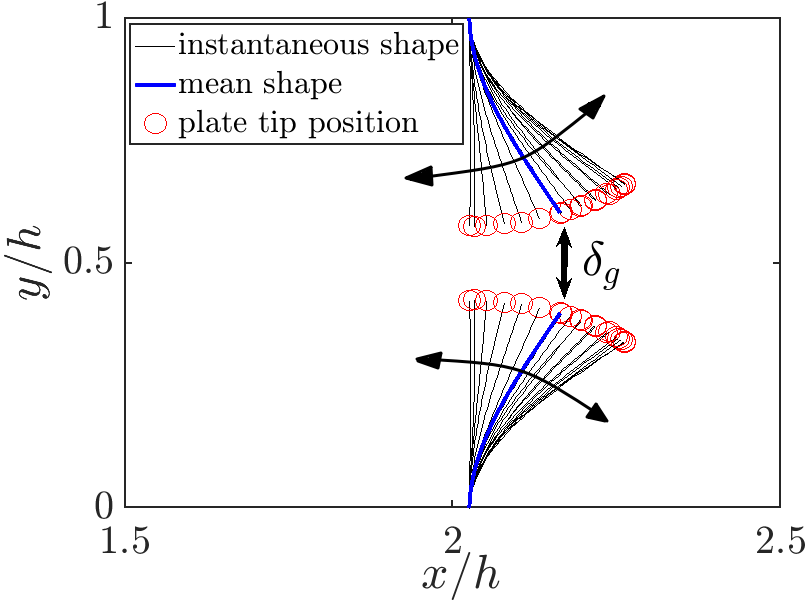
\includegraphics[width=1\linewidth]{Figures/def_shape3.png}
		\end{minipage}  
		\begin{minipage}[c]{0.49\linewidth}	
			\centering
			\begin{overpic}[width=1\linewidth]{Figures/gap_sig_4S_5S_5E_6D_6F.png} 
				\put(-180,95){{\parbox{1\linewidth}{$(a)$}}}	
				\put(-60,95){{\parbox{1\linewidth}{$(b)$}}}
			\end{overpic}
		\end{minipage} 
	\end{center}
	\vspace{-10px}
	\caption{(a) Stroboscopic images showing the plate reconfiguration for the steady inlet case with $Ca = 0.04$. The thick blue line represents the steady-state reconfigured shape, and the red circles mark the plates' tip position. (b) Time history of gap-width between the tip of the two plates normalized by the channel height ($\delta_g/h$).}
	\label{fig:del_g_vs_Ca_steady}
\end{figure}

We have tracked an additional scalar concentration field $\phi$ which is governed by an advection-diffusion equation as: 
\begin{equation*}
	{\partial\phi\over\partial t}+(\mathbf{u}_f-\mathbf{u}_m)\cdot\mathbf{\nabla}\mathbf{\phi} = \frac{1}{Re\cdot Sc}\nabla^2\mathbf{\phi},
\end{equation*}
where $\phi$ is the scalar concentration field, which ranges from 0 to 1, and $Sc=\nu_f/D$ is the Schimdt number, where $D$ is the mass diffusivity of the scalar concentration field. To solve the governing equations, we employed the finite volume method with a second-order accurate Euler-implicit scheme for temporal discretization, a second order vanLeer TVD scheme for spatial discretization of the convection and central differencing scheme with Gaussian integration to resolve diffusion terms. In our work, we ensure that the Courant number, based on the local velocity magnitude, the time-step of integration, and the length of the computational cell, remains below $0.2$. Our solution approach predicts the interface displacement and calculates the initial interface residual. This involves estimating the movement of the interface between the fluid and structure domains and determining the deviation from the initial position. Once the initial interface residual has been calculated, the algorithm initiates the fluid-structure interaction via a strongly coupled iterative procedure until the convergence criterion is met~\cite{Hrvoje2007, CampbellPaterson2011}. This iterative process is repeated under the Aitken dynamic relaxation approach until the desired tolerance level is achieved.
\begin{figure*}
	\begin{minipage}[c]{0.495\linewidth}
		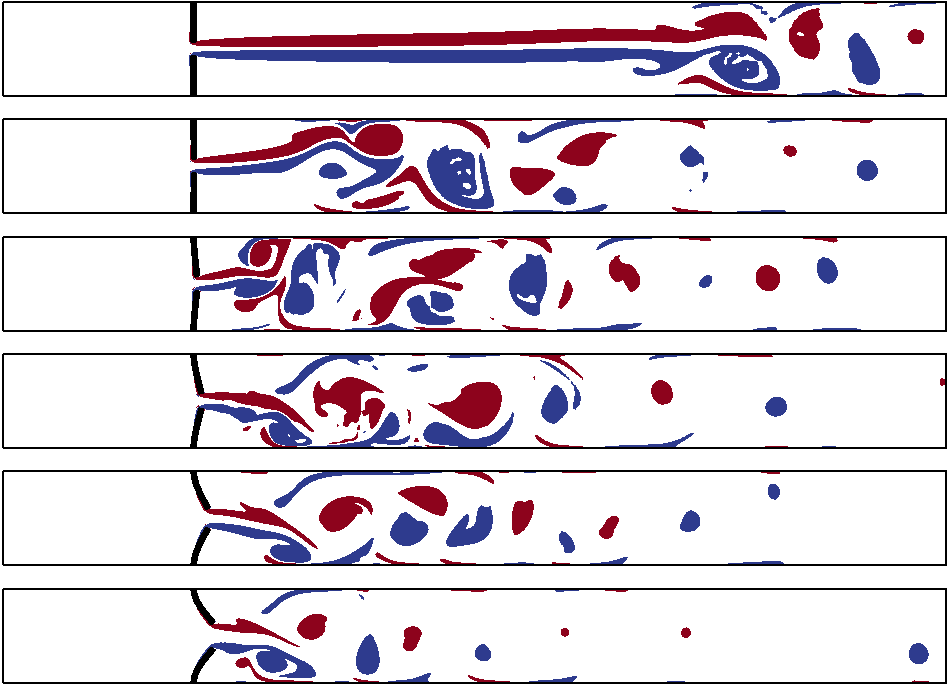
\includegraphics[width=1\linewidth]{Figures/vort_S_2500.png}
	\end{minipage}
	\begin{minipage}[c]{0.495\linewidth}		
		\begin{overpic}[width=1\linewidth]{Figures/scalar_S_2500.png}
			\put(-365,163){{\parbox{1\linewidth}{$rigid$}}}	
			\put(-355,131){{\parbox{1\linewidth}{$Ca=0.001$}}}
			\put(-355,100){{\parbox{1\linewidth}{$Ca=0.01$}}}	
			\put(-355,69){{\parbox{1\linewidth}{$Ca=0.02$}}}	
			\put(-355,38){{\parbox{1\linewidth}{$Ca=0.04$}}}
			\put(-355,6){{\parbox{1\linewidth}{$Ca=0.06$}}}
			\put(-130,-20){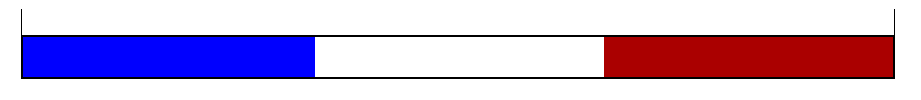
\includegraphics[width=0.45\linewidth]{Figures/legend_vortex.png}}
			\put(110,-20){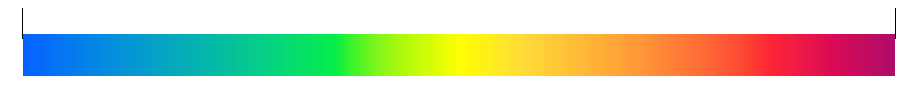
\includegraphics[width=0.45\linewidth]{Figures/legend_scalar.png}}
			\put(-255,-10){{\parbox{1\linewidth}{$-\infty$}}}	
			\put(-220,-10){{\parbox{1\linewidth}{$-5$}}}
			\put(-141,-10){{\parbox{1\linewidth}{$\infty$}}}
			\put(-200,-10){{\parbox{1\linewidth}{$\omega_z$}}}	
			\put(-180,-10){{\parbox{1\linewidth}{$5$}}}
			\put(-15,-10){{\parbox{1\linewidth}{$0$}}}
			\put(44,-10){{\parbox{1\linewidth}{$\phi$}}}
			\put(95,-10){{\parbox{1\linewidth}{$1$}}}
			\put(-125,190){{\parbox{1\linewidth}{$(b)$}}}
			\put(-390,190){{\parbox{1\linewidth}{$(a)$}}}
		\end{overpic}
	\end{minipage}  
	\vspace{0.5cm}
	\caption{Instantaneous (a) iso-contour plots of spanwise vorticity $(\omega_z)$ and (b) scalar concentration field for steady inlet flow case. The top to bottom panels are cases with rigid and flexible wall mounted plates with $Ca=0.001-0.06$.}
	\label{fig:contour_Ca}
\end{figure*}
For our investigation on fluid mixing, we have varied Young's Modulus $\mathcal{E}$ such that the plates's flexibility can be varied as a parameter. This parameter, Cauchy Number, $Ca=\rho_f U^2 h^3 b/{\mathcal{E}I}$ is defined as the ratio between fluid inertial force to the structural restoring force of the plate where $\rho_f$ is the fluid density, and $I=bw^3/12$ is the area moment of inertia of the structure. Due to the significance of structural forces and following prior works on microchannels involving flexible structures \citep{Vandenberghe2004}, we have varied $Ca$ in the range from $0$ to $0.06$, where $Ca=0$ is referred to as a rigid plate case. The time scale in this work is based on the fluid convection measure as $\tau \approx h/U$. The ratio of fluid density to structure density, in our case, is $\beta$ $=\rho_s b / \rho_f l = 5$. A pulsatile flow enters from the left (see Fig. \ref{fig:schematic}) composed of $(a)$ a steady flow of Reynolds number, $Re_{s} = 500$, based on channel height $h$ and mean free-stream inlet velocity $U$ and $(b)$ an oscillatory flow such that the inlet Reynolds Number, ${Re}(t)$ pulses with a sinusoidal functional shape of the waveform:
\begin{equation*}
	\centering
	{Re}(t) = {Re_s}\{1+0.5sin(2\pi St_f \tau)\}
	\label{eqn:pulse}
\end{equation*}
where $St_f (= f_f h/U)$ is the Strouhal number for an applied flow inlet frequency $f_f$. We have varied $St_f$ in the range $0$ to $32$, where $St_f=0$ represents a steady inlet condition. Such single-harmonic pulse waveform is previously used in many other experimental and numerical works about unsteady flows in channel and tube constrictions \cite{Giddens1984, hummel1989, carmo2019}. The inlet flow profile across the channel is set to mimic a fully developed parabolic nature as in Poiseuille channel flow and is expressed as $u_f(y)=6U\left(\frac{y}{h}\right)\left(1-\frac{y}{h}\right)$. The channel domain comprises a grid of $42480$ hexahedral cells as $360$ cells along the channel length and $118$ cells along its height. The thin plate structures are also computationally discretized into a hexahedral grid as $12$ cells along the thickness and $50$ cells along the plate height for each of the two plates. A zoom-in of the domain mesh grid at a section near the plates is shown in Figure \ref{fig:schematic}. To establish the most appropriate grid size for our simulations, we ascertain grid convergence analysis. We conducted a base simulation with $Re_s=500$ and steady flow conditions past the flexible plates with $Ca=0.04$ and $Sc=1$. In the simulation setup, the resolution in each direction was increased by a scale factor of $1.5$, leading us to utilize a total grid size of $480 \times 177$ cells, thus an increase in the overall number of points by approximately $3$ times. Consequently, we noted that head loss and the mixing index differed insignificantly with less than a variance rate amounting to no more than $1\%$, while the mixing index only varied very slightly with less than 1\% variation in results. 
\begin{figure*}
	\begin{minipage}[c]{0.42\linewidth}
		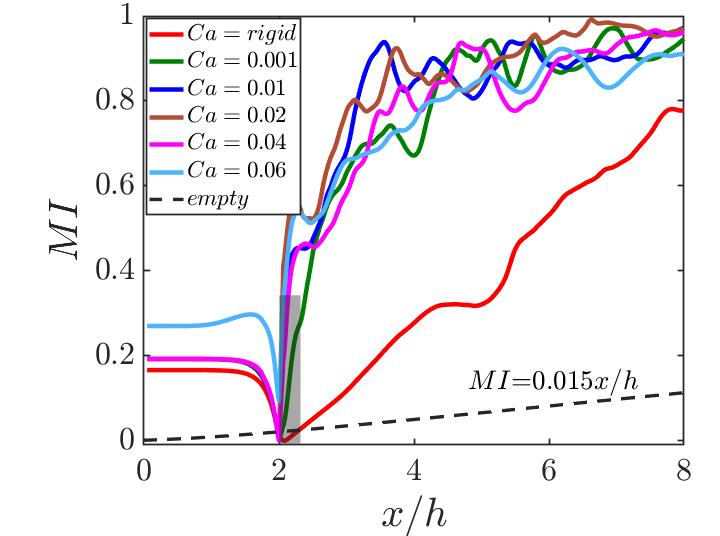
\includegraphics[trim={1.1cm 0 0 0},clip,width=1\linewidth]{Figures/MI_S_8h_ico.png}
	\end{minipage}
	\begin{minipage}[c]{0.41\linewidth}		
		\begin{overpic}[trim={1.1cm 0 0 0},clip,width=1\linewidth]{Figures/HL_S_ico.png}
			\put(-320,170){{\parbox{1\linewidth}{$(a)$}}}	
			\put(-95, 170){{\parbox{1\linewidth}{$(b)$}}}
		\end{overpic}
	\end{minipage}  
	%	\vspace{0.1cm}
	\caption{Time-averaged (a) mixing index $MI$ and (b) head loss $HL$ along the channel length in the downstream for steady inlet flow. The grey rectangle marks the location of plates in the channel.}
	\label{fig:MI_Ca}
\end{figure*}
Upon analyzing the results, we found that the flow and structural dynamics are well resolved at the present grid size. The grid refinement test and validation study on a similar simulation setup has been carried out extensively and exhibited in our prior work \cite{Self2019}. The velocity boundary conditions applied to the channel walls and flexible structure surfaces are no-slip and impermeable. The velocity gradients at the channel outlet boundary (on the right side) are set to zero, whereas the inlet velocity is set to pulsatile inflow, as described previously. Additionally, the interface velocity of the solid structure and the flow are the same. The pressure boundary conditions are set to zero gradients at channel walls, channel inlet and the fluid-solid interface and the channel outlet has ambient pressure ($zero$) conditions as a reference. We have focussed our study at the streamwise location $x=8h$ such that there would be no boundary reflections and the properties cushion out before leaving the channel.

\section{Results}
We have studied the mixing performance in a channel flow with passively oscillating flexible plates under impact the flow. Such plates under the action of an incoming flow may deform as lodging mode, regular VIV mode (vortex-induced vibration or flutter) or static reconfiguration mode as suggested by \cite{Zhang2020}. Based on the parameter range used, our cases lie in the phase space that exhibits static reconfiguration of the plates as shown in \cite{Zhang2020} where the plates comply with the flow, the projected area perpendicular to the flow reduces, and negligible flutter can be observed at later time (steady-state). In Figure \ref{fig:del_g_vs_Ca_steady}(a), stroboscopic visualization of the plates for steady inlet flow and $Ca=0.04$ are shown. The plate bends maximum at the tip in the streamwise direction, represented as the red circle in the figure. After the initial transients die down, the plates' tips flutter at very small amplitudes about a mean state (shown as the thick blue line). The gap opened between the plates creates spatial variation in the flow. In Figure \ref{fig:del_g_vs_Ca_steady}(b), the amplitude of gap between the two plates' tips, $(\delta_g)$ is shown with the time for different cases for reference. We can observe the effect of tip oscillations in different cases as varying gap amplitude due to pulsatile inlet conditions. We can also note the higher bending state for increased $Ca$ cases.

In Figure \ref{fig:contour_Ca}(a), instantaneous iso-contours of flow vorticity (into the plane, $\omega_z=\nabla\times u_f$ ) for rigid plate and flexible plate cases are shown. The flow accelerates through the gap between the plates to form a jet-like flow. In rigid plate cases, this jet-like flow is observed for long lengths beyond which the flow instabilities take place. However, this jet length breaks up earlier in flexible plate case due to the plates' tiny tip-oscillations, which act as a source for perturbation into this jet-like flow and generate oppositely rotating vortex structures which spread out in the channel downstream in alternating fashion. These vortex structures, under the effect of inlet inertia, get advected in the downstream direction and lose momentum by diffusion into the flow, which in turn act as a `stirring effect' and induce fluid mixing.
\begin{figure*}
	\begin{minipage}[c]{0.495\linewidth}
		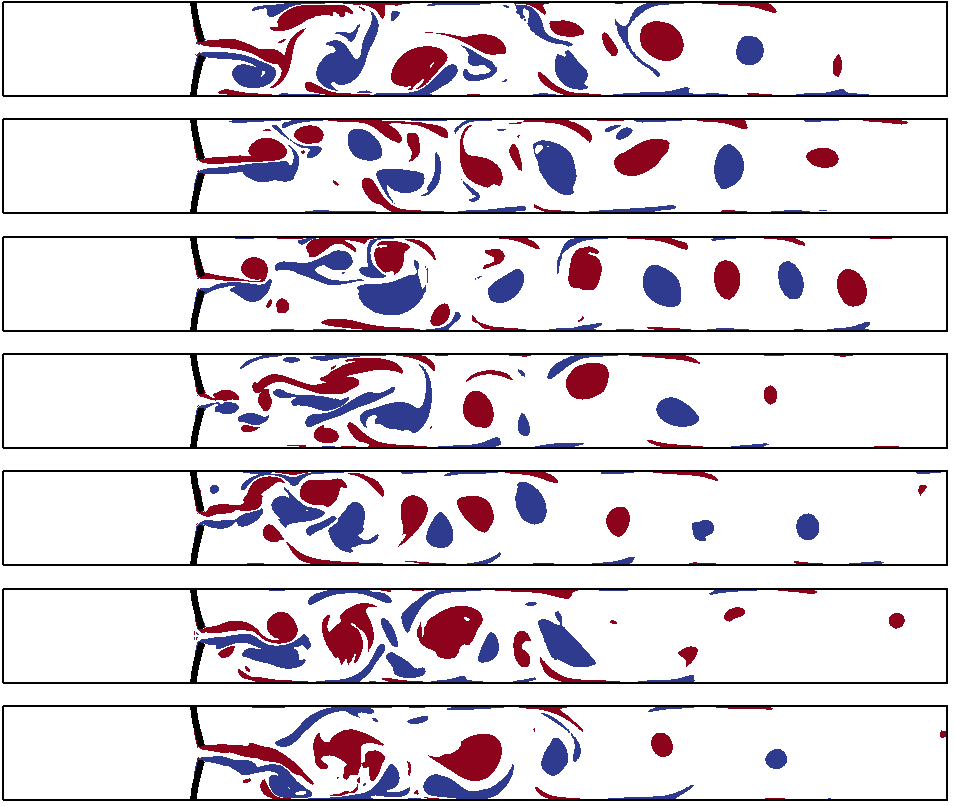
\includegraphics[width=1\linewidth]{Figures/vort_4_2500.png}
	\end{minipage}
	\begin{minipage}[c]{0.495\linewidth}		
		\begin{overpic}[width=1\linewidth]{Figures/scalar_4_2500.png}
			\put(-362,190){{\parbox{1\linewidth}{$St_f=1$}}}	
			\put(-362,159){{\parbox{1\linewidth}{$St_f=2$}}}
			\put(-362,128){{\parbox{1\linewidth}{$St_f=4$}}}	
			\put(-362,98){{\parbox{1\linewidth}{$St_f=8$}}}	
			
			\put(-360,66){{\parbox{1\linewidth}{$St_f=16$}}}
			\put(-360,35){{\parbox{1\linewidth}{$St_f=32$}}}
			\put(-360,3){{\parbox{1\linewidth}{$steady$}}}
			%	\put(-60,105){{\parbox{1\linewidth}{\rotatebox{87}{$transiton$}}}}
			\put(-130,-20){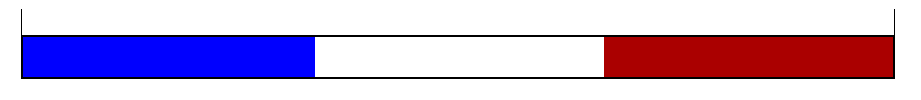
\includegraphics[width=0.45\linewidth]{Figures/legend_vortex.png}}
			\put(125,-20){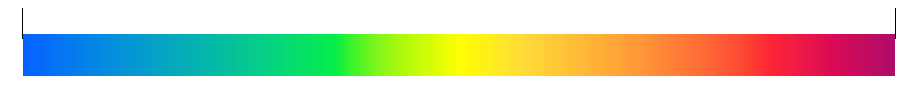
\includegraphics[width=0.45\linewidth]{Figures/legend_scalar.png}}
			\put(-252,-10){{\parbox{1\linewidth}{$-\infty$}}}	
			\put(-220,-10){{\parbox{1\linewidth}{$-5$}}}
			\put(-200,-10){{\parbox{1\linewidth}{$\omega_z$}}}
			\put(-145,-10){{\parbox{1\linewidth}{$\infty$}}}	
			\put(-180,-10){{\parbox{1\linewidth}{$5$}}}
			
			\put(1,-10){{\parbox{1\linewidth}{$0$}}}
			\put(53,-10){{\parbox{1\linewidth}{$\phi$}}}
			\put(110,-10){{\parbox{1\linewidth}{$1$}}}
			
			\put(-125,217){{\parbox{1\linewidth}{$(b)$}}}
			\put(-385,217){{\parbox{1\linewidth}{$(a)$}}}
		\end{overpic}
	\end{minipage}
	\vspace{0.6cm}
	\caption{Instantaneous contour plots of (a) spanwise vorticity and (b) scalar concentration field for $Ca=0.02$ case. The top to bottom panels are cases with pulsatile inlet at $St_f=1,2,4,8,16,32 \, and$ steady flow inlet.}
	\label{fig:contour_St}
\end{figure*} 
In Figure \ref{fig:contour_Ca}(b), the scalar concentration field is shown which, initially, is distinctly separated by an interface about the midline along the channel length, but as the flow progresses, the scalar field diffuses into one another across the interface layer. In the rigid plate case, the scalar fields remain unmixed until jet-like flow oscillates at a later downstream location when the vortex structures begin to detach. The vortex structures agitate the flow, and the layer separating the two scalars stretches in length. The larger `interface length' causes the diffusion process to act more efficiently and thereby increases the mixing process. With the increase in plate flexibility ($Ca=0.001-0.06$), the jet-like flow breakups early in the downstream larger count of advecting vortex structures can be observed. The aforementioned `stirring effect' caused by these vortex rolls due to increased interface layers induces the mixing of the scalars towards homogeneity. The alternate rolling of clockwise and counter-clockwise vortices entrain scalar alternately from the top wall side and bottom wall side. This entrainment from both sides evolves into localised mixing zones, which advect under the effect of inertia. Such local mixing zones cause agitation in the flow and hence accelerate the diffusive mixing.
\begin{figure*}
	\begin{minipage}[c]{0.44\linewidth}
		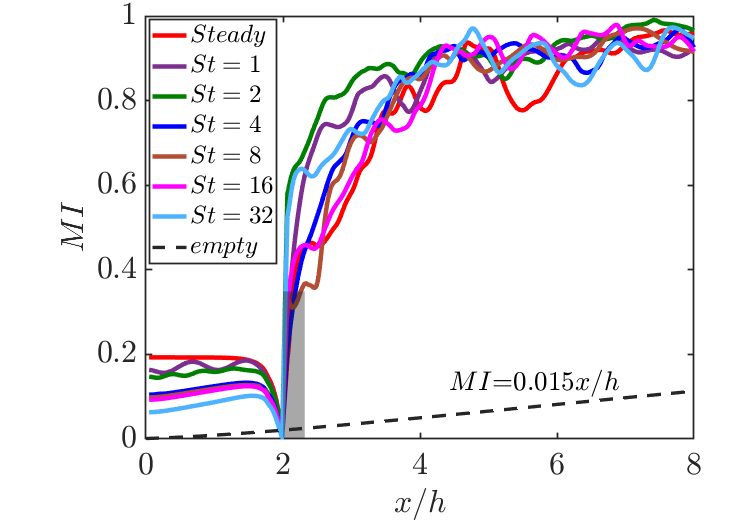
\includegraphics[width=1\linewidth,trim={1cm 0 0 0},clip]{Figures/MI_5_ico.png}
	\end{minipage}
	\begin{minipage}[c]{0.43\linewidth}		
		\begin{overpic}[width=1\linewidth,trim={1cm 0 0 0},clip]{Figures/HL_5_ico.png}
			\put(-320,170){{\parbox{1\linewidth}{$(a)$}}}	
			\put(-100,170){{\parbox{1\linewidth}{$(b)$}}}
		\end{overpic}
	\end{minipage} %	\vspace{0.5cm}
	\caption{Time averaged (a) mixing index $MI$ and (b) head loss $HL$ along the channel length in the downstream for flexible plate case with $Ca=0.04$. The grey rectangle marks the location of plates in the channel.}
	\label{fig:MI_St}
\end{figure*}
To evaluate the mixing performance in channel flows, various metrics have been used in the past \citep{Danckwerts1952,Kockmann2006,Liscinsky1993}. In our work, we have used one of the most widely used metrics called `Mixing Index' ($MI$), which is evaluated along the streamwise location as:
	\begin{eqnarray*}
	MI(x)=1-\sqrt{\frac{\sigma(x)^2}{{\sigma^2_{max}}}}
		\\
	where \quad \sigma(x)=\sqrt{{1\over h} \int_{0}^{h} [\phi(x,y)-\phi_m]^2 \,dy}\\
	\end{eqnarray*}
where $\sigma(x)$ is the standard deviation of the vertically integrated scalar field across the channel height, $\phi_m$ is the scalar concentration value for a completely mixed solution or mean of the scalar concentration field range and $\sigma_{max}$ is the maximum deviation in the scalar concentration field within the fluid domain. As per the expression, $MI=0$ represents a completely unmixed field, whereas $MI=1$ means full mixing with completely homogenised scalar concentration. We have also computed vertically integrated mechanical head loss $(HL)$ in the flow evaluated along the streamwise location during the mixing process as:
\begin{eqnarray*}
	\mathcal{H}^*(x)=\frac{\mathcal{H}(x)}{\rho_f U^2}=\frac{1}{h}\int_{0}^{h}[p(x,y)+{1\over2}  u^2(x,y)]\,dy \\ \\Head \: Loss, HL(x) = \mathcal{H}^*(0)-\mathcal{H}^*(x)
\end{eqnarray*}
In Figure \ref{fig:MI_Ca}(a), $MI(x)$ a for steady inlet flow is shown for rigid and flexible plate cases. The grey shaded rectangle at $x/h=2$ marks the location of the plates in the channel. The $MI$ suddenly shoots high next to the plates ($2<x/h<4$) for flexible plate cases, unlike the rigid plate case, where the $MI$ increases gradually along the channel length. This is due to the lower entrainment of the scalar concentration field in the rigid plate case because of the inertia-driven jet-like flow next to the plates, as discussed above. With increasing $Ca$, the $MI$ shows an even steeper curve and exhibits the fluid mixing early in the channel location. We have also shown the $MI$ along the channel length in an empty channel, i.e. with no obstacles for reference. In Figure \ref{fig:MI_Ca}(b), the total mechanical head loss, $HL$, is shown along the channel streamwise direction. The $HL$ jumps suddenly at the plates' location to a value based on the plates' flexibility. Most flexible case ($Ca=0.06$) show minimum $HL$, whereas the rigid plates case offers the highest $HL$ among all the cases.

To understand the effect of pulsatile inlet conditions in the flow dynamics and mixing performance, we have shown the instantaneous vorticity contour in Figure \ref{fig:contour_St} for $Ca=0.04$ with $St_f=1-32$, and steady inlet. In comparison to the steady inlet conditions, an increase in flow pulsation generates even more complex vorticity dynamics due to the plates' tip oscillation.
In Figure \ref{fig:MI_St}, $MI$ and $HL$ are shown along the downstream location. $MI$ increases earliest in the channel in the case with flow inlet at $St_f=2$ whereas, the $HL$ remains nearly indifferent to the effect of pulsatile inlet flow.

\begin{figure*}
	\begin{center}
		\begin{minipage}[c]{0.44\linewidth}
			\begin{overpic}[width=1\linewidth]{Figures/MI_8h_HL.png}
			\end{overpic}
		\end{minipage}
		\begin{minipage}[c]{0.44\linewidth}
			\begin{overpic}[width=1\linewidth]{Figures/CoP_8h.png}
				\put(-320,170){{\parbox{1\linewidth}{$(a)$}}}	
				\put(-105,170){{\parbox{1\linewidth}{$(b)$}}}
				\put(-60,7){{\parbox{1\linewidth}{$(rigid)$}}}
			\end{overpic}
		\end{minipage}
	\end{center}
		\vspace{-0.5cm}
	\caption{(a) Performance comparison in terms of mixing index and head loss $HL$ for the different cases in this work. The solid mark corresponds to the steady inlet flow case. A zoom-in of each of the clusters based on the plates' flexibility is shown separately in the Appendix section for $St_f$ cases. (b) Coefficient of performance $CoP$ for increasing $Ca$ and different $St_f$ cases.}
	\label{fig:MImax_HL}
\end{figure*}


In Figure \ref{fig:MImax_HL}(a), we have summarised the mixing performance of all the cases studied in our work. We have shown $MI$ and $HL$ attained at the channel length $x/h=8$ for cases with different $Ca$ and $St_f$. The clusters of data points arranged according to the Cauchy numbers $(Ca)$ can be observed where the solid marker point corresponds to the steady inlet conditions. 
Among these summarized data points, the most flexible plate case ($Ca=0.06$) offers significant mixing at considerably low $HL$ compared to all other cases. However, even more mixing can be achieved at the cost of a slight increase in $HL$ in the case of $Ca=0.04$. This fluid mixing can be fine-tuned to the best performance by modulating the inlet flow pulsation, such as in the case with $Ca=0.06,\, St_f=32$. In contrast, the mixing performance of the flexible plate cases is significantly better than that of rigid plate cases.


%%
A primary goal when designing a small mixer is to make it as small as possible while ensuring effective mixing. To find out the "compactness" of the channel mixer with wall-mounted plates, we can look at how long a mixer channel without any plates (or an empty channel) would need to be to achieve the same mixing level as the channel with plates at the streamwise location $x/h = 8$. Similarly, to understand efficiency losses in such channel mixers is to find the length of the empty channel that experiences the same loss as one with plates. These equivalent channel lengths for an empty channel case are separately quantified for mixing length $E_M$ and for head loss $E_H$. To estimate these equivalent lengths, we find that the mixing index and head loss in the empty channel with steady inlet flow (i.e., with no plate) can be very accurately fit as a linear profile, i.e., $MI = 0.015x/h$ and $HL(x)=0.0032x/h$, in our setup (see Figure \ref{fig:MI_Ca}). From this understanding, we can introduce a Coefficient of Performance (CoP) for the mixer, calculated as the ratio of equivalent lengths for mixing and loss (i.e., $CoP = E_M/E_H$) \citep{Aaron2019}. This coefficient helps us see how much the mixing improves in relation to the increase in efficiency loss for a mixer compared to a design without any plates. We have provided the equivalent lengths and Coefficient of Performance for some instances in Table 1. This data shows how adding plates can make a mixer more compact and offers a way to compare different mixer designs. In Figure \ref{fig:MImax_HL}(b), we have shown the $CoP$ for different $Ca$ and $St_f$ cases. We can confirm that the flexible plates offer better mixer performance. In contrast, the pulsatile inlet does not offer any significant improvement in overall mixing performance compared to the steady inlet cases because of the head loss incurred by the pulsatile inlet conditions. However, among all the cases, $Ca=0.06$ with $St_f=32$ offers the best fluid mixing in our setup.

\begin{table*}
	\caption{\label{tab:table1}Equivalent lengths for mixing and head loss and corresponding coefficient of pressure for our cases.}
	\begin{ruledtabular}
		\begin{tabular}{ccccccc}
			\multicolumn{2}{c}{Case} & MI(8) & HL(8) & $E_M$ & $E_H$ & $CoP$\\
			\hline \\
%		\multicolumn{2}{c}{Case} & MI(8) & HL(8) & $E_M$ & $E_H$ & $CoP$\\
		rigid & steady& 0.886 &1.625 &59.08 &507.80 & 0.116\\
		$0.01$ & steady&  0.973& 1.660 &64.87 &518.85 &  0.125\\
		$0.04$ & steady&  0.962& 0.875 &64.16 &273.35 & 0.235\\
		$0.06$ & steady&  0.908& 0.453 &60.51 &141.53 & 0.427\\
		$0.06$ & $St_f$=8& 0.887& 0.459 &62.53 &143.44 & 0.412\\
		$0.06$ & $St_f$=32&0.896 &0.445 &59.73 &138.90 & 0.430\\
		\end{tabular}
	\end{ruledtabular}
\end{table*}

\section{Summary}
We have conducted computer simulations to analyze the mixing of two initially separated fluids in a channel mixer characterized by the parameters Reynolds number, $Re=500$ and Schmidt number, $Sc=1$. The design of this channel incorporates two flexible plates affixed to its walls. As the fluid flows, these plates experience bending and demonstrate tip oscillations (about a mean position), contributing to the mixing process. Additionally, we have also examined the impact of periodic inlet conditions on mixing outcomes. We have used standard metrics to determine both the efficiency of mixing and the associated mechanical head loss. Our observations reveal that flexible plates not only enhance the mixing quality when compared to rigid plates but also lead to reduced head loss. Whereas, in scenarios with pulsatile inlet conditions, mixing results varied based on the $St_f$ value and were accompanied by an increased head loss. To provide a comprehensive evaluation of mixing performance, taking into account both the quality of mixing and the head loss, we have compared our configuration with a scenario involving an empty channel (with no obstacles). We utilized equivalent empty channel lengths ($E_M$ and $E_H$) for this comparison, aiming to achieve metrics comparable to the channel equipped with plates. Subsequently, we computed the coefficient of performance, defined as $CoP=E_M/E_H$, for all examined scenarios to rank our setups based on their mixing performance. The optimal mixing performance was observed in the scenario characterized by $Ca=0.06$ and $St_f=32$, followed closely by $Ca=0.06$ with a steady inlet condition. In conclusion, greater flexibility in the plates leads to better mixing performance. This performance can be marginally refined by using pulsatile inlet in some cases.
Nevertheless, our study has its limitations. Primarily, the geometric design of the channel mixer used is simplistic, representing a straight, two-dimensional channel. In practical applications, mixers might possess more intricate, duct-like channels where three-dimensional flow dynamics are significant. Such three-dimensional attributes could potentially alter the dynamics of the elastic plates and the overarching flow dynamics. Future research could explore the influence of plates' geometry and their location within the channel on mixing efficiency.


\section{Acknowledgement}
We thank our fellow members of TuRbulent Interfaces And Dispersion (TRIAD), IIT Kharagpur, for their support. We acknowledge research grants from the Board of Research and Nuclear Science(BRNS), INSPIRE and MATRICS sponsored by the Science and Engineering Research Board of the Government of India. We sincerely thank Param Shakti for computing resources developed under the National Supercomputing Mission at IIT Kharagpur, India.



%
%\begin{ruledtabular}
%\begin{tabular}{cccccccc}
% &$r_c$ (\AA)&$r_0$ (\AA)&$\kappa r_0$&
% &$r_c$ (\AA) &$r_0$ (\AA)&$\kappa r_0$\\
%\hline
%Cu& 0.800 & 14.10 & 2.550 &Sn\footnotemark[1]
%& 0.680 & 1.870 & 3.700 \\
%Ag& 0.990 & 15.90 & 2.710 &Pb\footnotemark[2]
%& 0.450 & 1.930 & 3.760 \\
%Au& 1.150 & 15.90 & 2.710 &Ca\footnotemark[3]
%& 0.750 & 2.170 & 3.560 \\
%Mg& 0.490 & 17.60 & 3.200 &Sr\footnotemark[4]
%& 0.900 & 2.370 & 3.720 \\
%Zn& 0.300 & 15.20 & 2.970 &Li\footnotemark[2]
%& 0.380 & 1.730 & 2.830 \\
%Cd& 0.530 & 17.10 & 3.160 &Na\footnotemark[5]
%& 0.760 & 2.110 & 3.120 \\
%Hg& 0.550 & 17.80 & 3.220 &K\footnotemark[5]
%&  1.120 & 2.620 & 3.480 \\
%Al& 0.230 & 15.80 & 3.240 &Rb\footnotemark[3]
%& 1.330 & 2.800 & 3.590 \\
%Ga& 0.310 & 16.70 & 3.330 &Cs\footnotemark[4]
%& 1.420 & 3.030 & 3.740 \\
%In& 0.460 & 18.40 & 3.500 &Ba\footnotemark[5]
%& 0.960 & 2.460 & 3.780 \\
%Tl& 0.480 & 18.90 & 3.550 & & & & \\
%\end{tabular}
%\end{ruledtabular}
%\footnotetext[1]{Here's the first, from Ref.~\onlinecite{feyn54}.}
%\footnotetext[2]{Here's the second.}
%\footnotetext[3]{Here's the third.}
%\footnotetext[4]{Here's the fourth.}
%\footnotetext[5]{And etc.}
%\end{table}



%\appendix

%\section{Appendixes}

%\nocite{*}
\bibliography{pre2.bib}% Produces the bibliography via BibTeX.

\newpage

\section*{Appendix}
\appendix

%\section{Flow features behind plates}
\onecolumngrid
%\singlespacing
In Figure~\ref{fig:vel_Q}, instantaneous streamwise velocity contour (left) and Q-criterion based vortex structures are shown. Using $Q$-criterion, strong vortices in the flow (with $Q>0$) can be detected during run time calculations~\cite{Hunt1994, Hussain1995, Holmes2012, Rowley2014}. The vortex dominated zones and the strained zones can be identified by $Q>0$ and $Q<0$, respectively. We can observe accelerated flow through the gap and multiple recirculation zones attached in the downstream side. Figure~\ref{fig:vel_pro} indicates the amplitude of flow speed up and subsequent decay along the channel length. Figure \ref{fig:vel_Q} shows the zoomed-in view of each clusters of data points shown in \ref{fig:MImax_HL}(a) which indicates effect of $St_f$ on mixing performance.
\begin{figure}[h]
		\begin{minipage}[c]{0.09\linewidth}	
		
\includegraphics[width=1\linewidth]{blank.png} 
	\end{minipage}
	\begin{minipage}[c]{0.45\linewidth}		
		\begin{overpic}[width=1\linewidth]{Figures/1S1D3S3D5S5D_Umag.png}
			\put(-145,107){{\parbox{1\linewidth}{\footnotesize{$rigid, steady$}}}}	
			\put(-145,86){{\parbox{1\linewidth}{\footnotesize{$rigid,St_f=8$}}}}
			\put(-145,66){{\parbox{1\linewidth}{\footnotesize{$Ca=0.01, steady$}}}}	
			\put(-145,45){{\parbox{1\linewidth}{\footnotesize{$Ca=0.01, St_f=8$}}}}	
			\put(-145,25){{\parbox{1\linewidth}{\footnotesize{$Ca=0.04, steady$}}}}
			\put(-145,4){{\parbox{1\linewidth}{\footnotesize{$Ca=0.04, St_f=8$}}}}
			%	\put(-60,105){{\parbox{1\linewidth}{\rotatebox{87}{$transiton$}}}}
			\put(100,-20){
\includegraphics[width=0.45\linewidth]{Figures/leg_U.png}}
			\put(315,-20){
\includegraphics[width=0.45\linewidth]{Figures/leg_Q.png}}
			\put(35,-10){{\parbox{1\linewidth}{$u_x/U$}}}	
			\put(-14,-10){{\parbox{1\linewidth}{$-0.5$}}}
			\put(253,-8){{\parbox{1\linewidth}{$Q$}}}	
			\put(87,-10){{\parbox{1\linewidth}{$0.5$}}}
			\put(200,-10){{\parbox{1\linewidth}{$-10$}}}
			\put(305,-10){{\parbox{1\linewidth}{$10$}}}
			\put(-120,122){{\parbox{1\linewidth}{$(a)$}}}
			\put(120,122){{\parbox{1\linewidth}{$(b)$}}}
		\end{overpic}
	\end{minipage}
	\begin{minipage}[c]{0.45\linewidth}
		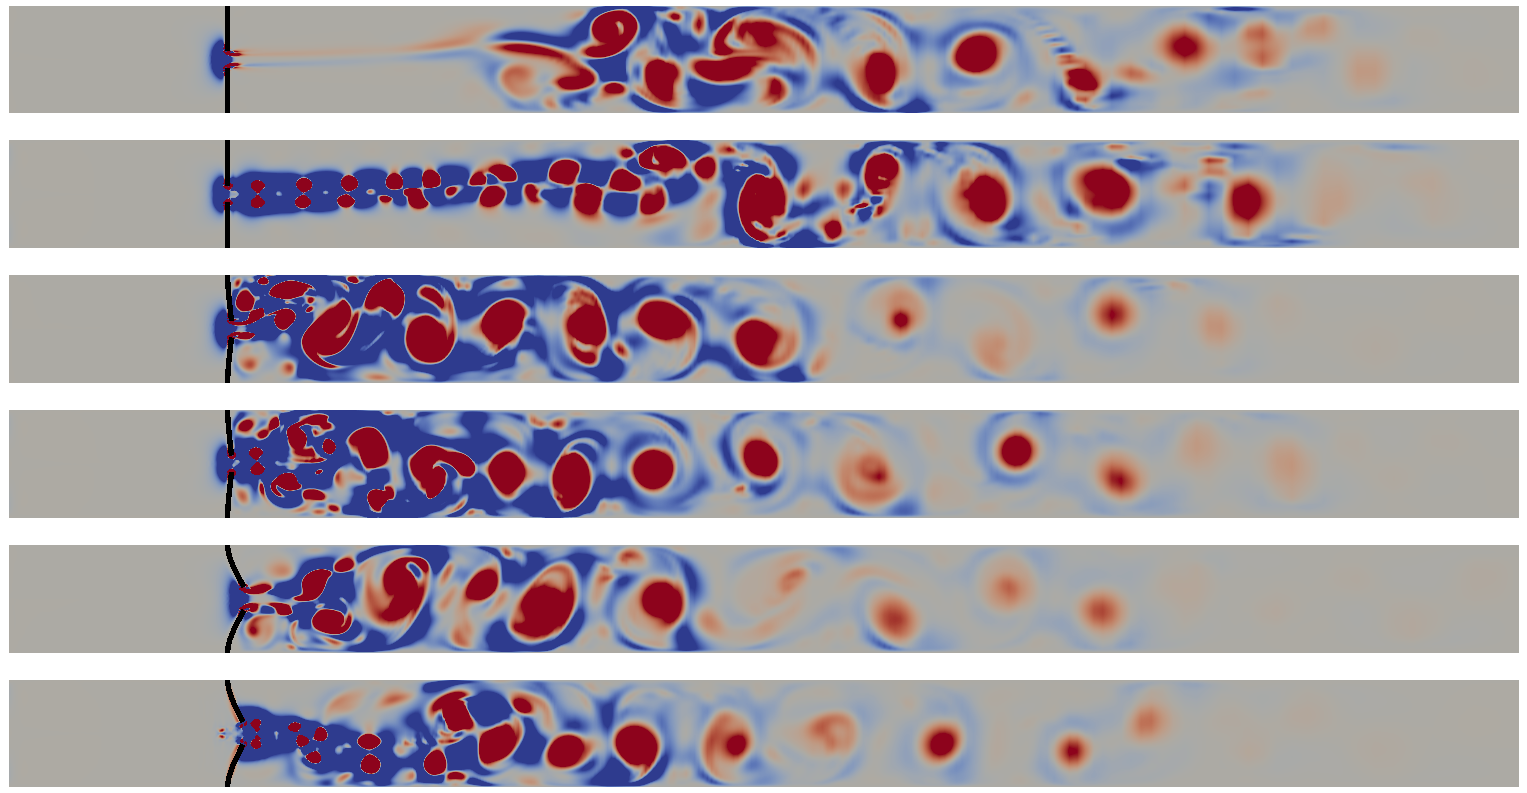
\includegraphics[width=1\linewidth]{Figures/1S1D3S3D5S5D_Q.png} 
	\end{minipage}\vspace{0.6cm}
	\caption{(a) Instantaneous streamwise velocity contour for different cases. (b) Q-criterion based vortex structures are shown.}
	\label{fig:vel_Q}
\end{figure}
\begin{figure}[h]
			\begin{minipage}[c]{0.09\linewidth}	
		
\includegraphics[width=1\linewidth]{blank.png} 
	\end{minipage}
	\begin{minipage}[c]{0.45\linewidth}
		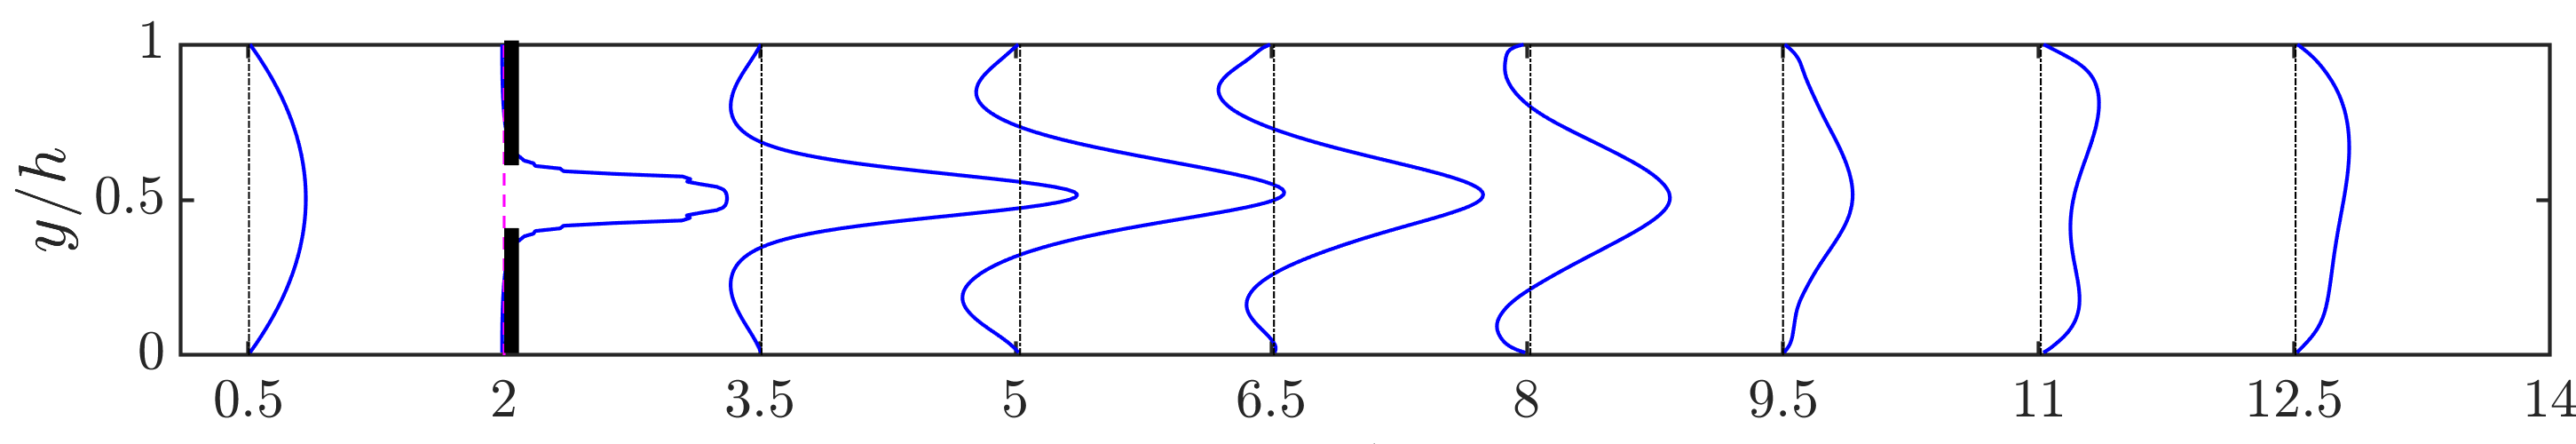
\includegraphics[width=1\linewidth]{velpro/1S_parabolic_velpro.png} 
		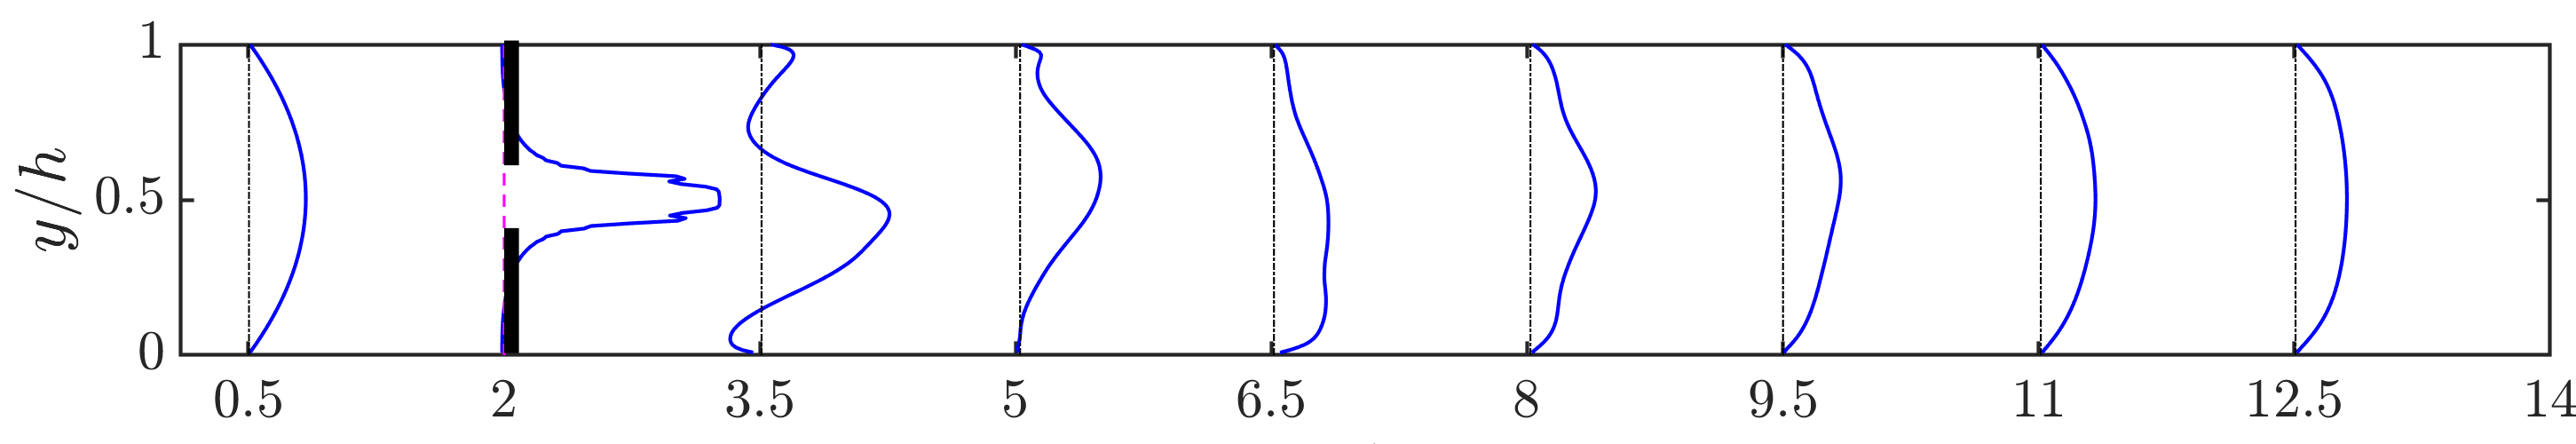
\includegraphics[width=1\linewidth]{velpro/4S_parabolic_velpro.png} 
		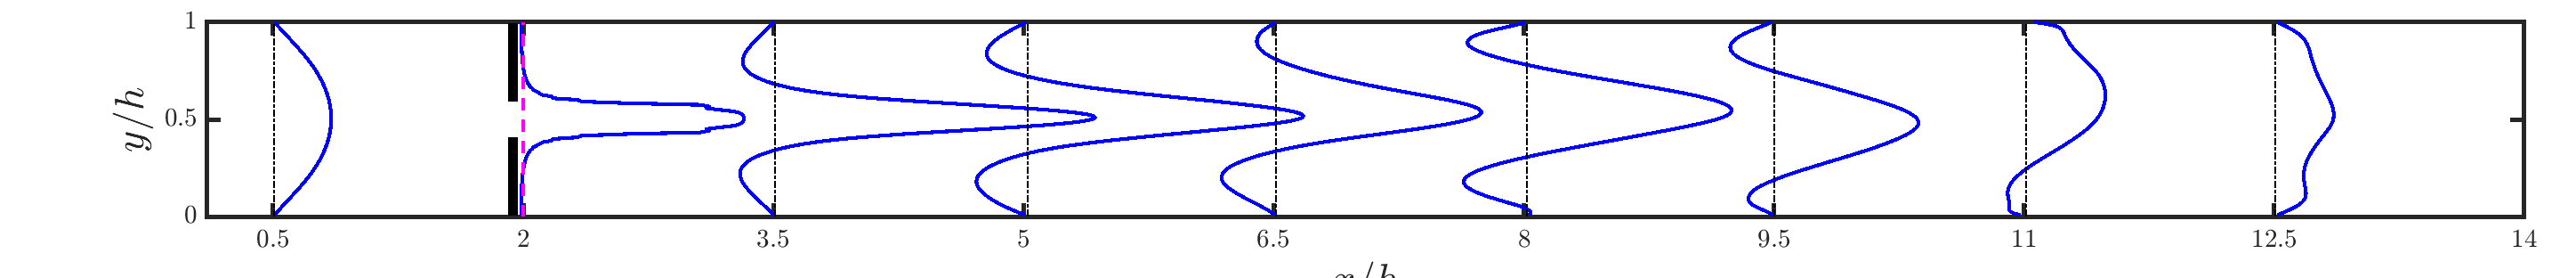
\includegraphics[width=1\linewidth]{velpro/1D_velpro.png} 
		\includegraphics[width=1\linewidth]{velpro/4D_velpro.png} 
	\end{minipage}
	\begin{minipage}[c]{0.45\linewidth}
		\includegraphics[width=1\linewidth,height=1.41cm]{midline/1S_midline_parabolic.png}
		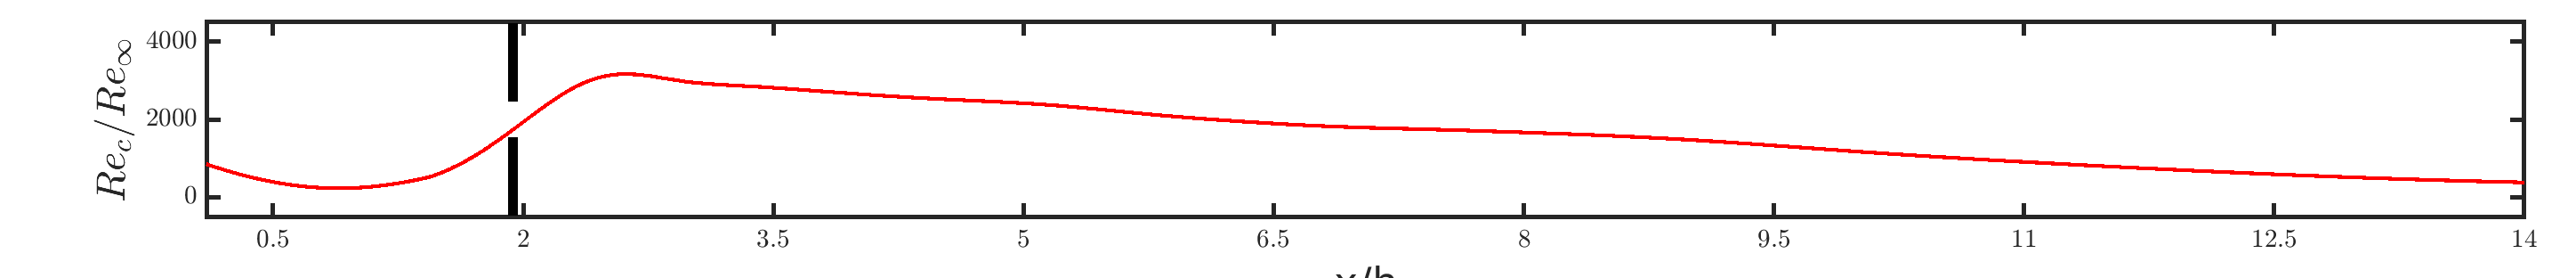
\includegraphics[width=1\linewidth,height=1.41cm]{midline/1D_midline.png}
		\includegraphics[width=1\linewidth,height=1.41cm]{midline/4S_midline_parabolic.png}
		\begin{overpic}[width=1\linewidth,height=1.41cm]{midline/4D_midline.png}
			\put(-375,139){{\parbox{1\linewidth}{\footnotesize{$rigid, steady$}}}}	
			\put(-375,100){{\parbox{1\linewidth}{\footnotesize{$rigid,St_f=8$}}}}
			\put(-380,60){{\parbox{1\linewidth}{\footnotesize{$Ca=0.02, steady$}}}}	
			\put(-380,18){{\parbox{1\linewidth}{\footnotesize{$Ca=0.02, St_f=8$}}}}	
			\put(-355,160){{\parbox{1\linewidth}{$(a)$}}}
			\put(-112,160){{\parbox{1\linewidth}{$(b)$}}}
		\end{overpic}
	\end{minipage}	
	\caption{(a) Time-averaged velocity profiles across the channel at six different streamwise locations. (b) Time-averaged center-line Reynolds number ($Re_c$) along the channel's length normalized with  ($Re_{S}$).}
	\label{fig:vel_pro}
\end{figure}
\vspace{0.45cm} 
\begin{figure}
	\begin{center}
		\begin{minipage}[c]{0.3\linewidth}
			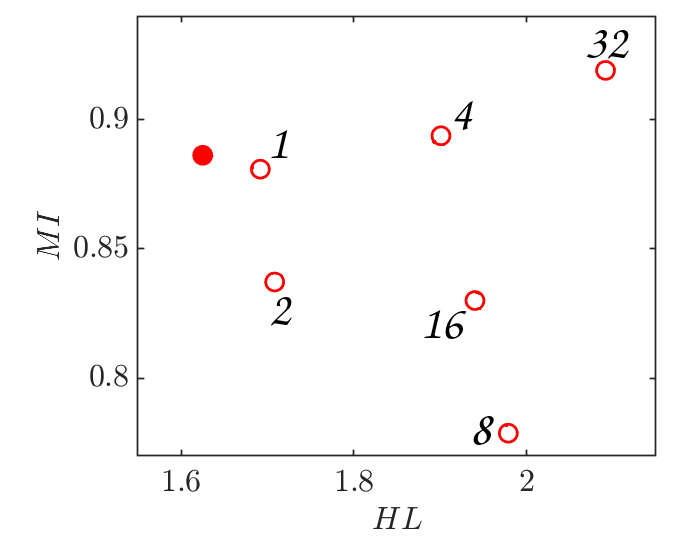
\includegraphics[width=1\linewidth,trim=0.5cm 0cm 0cm 0cm,clip]{Figures/MI_8h_HL_1.png}
		\end{minipage}
		\begin{minipage}[c]{0.3\linewidth}
			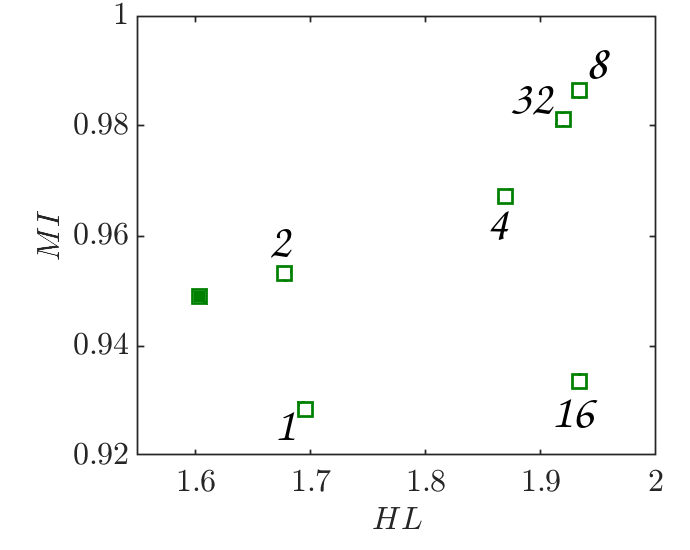
\includegraphics[width=1\linewidth,trim=0.5cm 0cm 0cm 0cm,clip]{Figures/MI_8h_HL_2.png}
		\end{minipage}
		\begin{minipage}[c]{0.3\linewidth}
			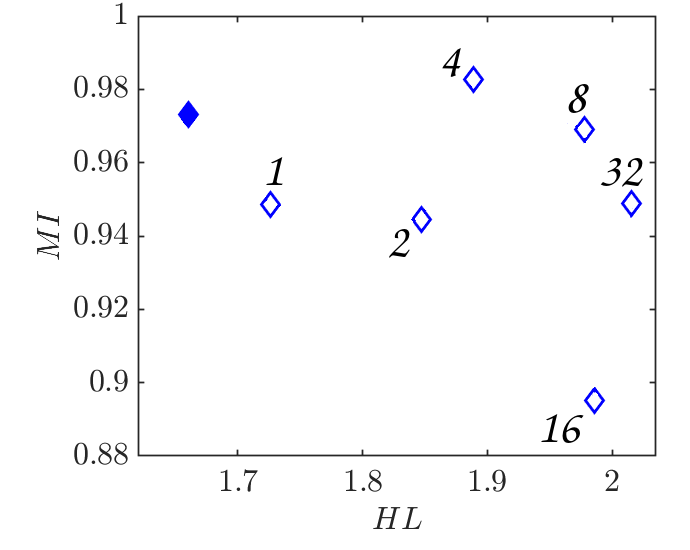
\includegraphics[width=1\linewidth,trim=0.5cm 0cm 0cm 0cm,clip]{Figures/MI_8h_HL_3.png}
		\end{minipage}\\
		\begin{minipage}[c]{0.3\linewidth}
			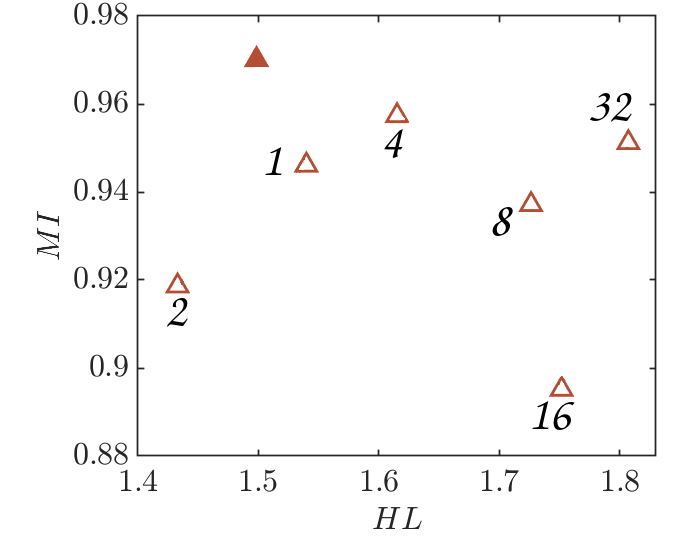
\includegraphics[width=1\linewidth,trim=0.5cm 0cm 0cm 0cm,clip]{Figures/MI_8h_HL_4.png}
		\end{minipage}
		\begin{minipage}[c]{0.3\linewidth}
			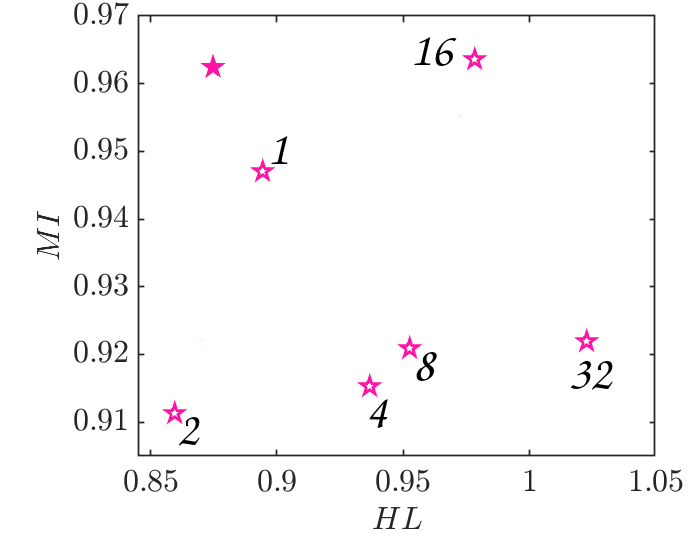
\includegraphics[width=1\linewidth,trim=0.5cm 0cm 0cm 0cm,clip]{Figures/MI_8h_HL_5.png}
		\end{minipage}
		\begin{minipage}[c]{0.3\linewidth}
			\begin{overpic}[width=1\linewidth,trim=0.5cm 0cm 0cm 0cm,clip]{Figures/MI_8h_HL_6.png}
				\put(-325,235){{\parbox{1\linewidth}{$rigid$}}}	
				\put(-158,235){{\parbox{1\linewidth}{$Ca=0.001$}}}
				\put(-8,235){{\parbox{1\linewidth}{$Ca=0.01$}}}	
				\put(-335,25){{\parbox{1\linewidth}{$Ca=0.02$}}}	
				\put(-110,25){{\parbox{1\linewidth}{$Ca=0.04$}}}	
				\put(40,25){{\parbox{1\linewidth}{$Ca=0.06$}}}	
			\end{overpic}
		\end{minipage}\vspace{-0.4cm}
	\end{center}
	\caption{Zoom-in of each clusters of data points shown in Figure \ref{fig:MImax_HL}(a). The solid marker corresponds to the steady inlet case, whereas the rest hollow markers are for periodic inlet condtions and $St_f$ value is shown near each data point.}
	\label{fig:MImax_HL2_zoom}
\end{figure}

\end{document}



%
% ****** End of file aipsamp.tex ******